\documentclass[11pt,a4paper]{article}
\usepackage[utf8]{inputenc}
\usepackage[vietnamese]{babel}
\usepackage{amsmath,amssymb}
\usepackage[version=4]{mhchem}
\usepackage{geometry}
\geometry{top=1.5cm,bottom=1.2cm,left=1.4cm,right=1.4cm,headheight=28pt,headsep=12pt,footskip=18pt}
\usepackage{graphicx}
\usepackage{xcolor}
\usepackage{tabularx}
\usepackage{array}
\usepackage{tikz}
\usepackage{fancyhdr}
\usepackage{enumitem}

\definecolor{hfRed}{HTML}{D32F2F}
\definecolor{hfGreen}{HTML}{8BC390}
\definecolor{mainGreen}{HTML}{2E7D32}

\usepackage{ex_test}

\pagestyle{fancy}
\fancyhf{}
\renewcommand{\headrulewidth}{0.75pt}
\renewcommand{\headrule}{\hbox to\headwidth{\color{hfGreen}\leaders\hrule height \headrulewidth\hfill}}
\renewcommand{\footrulewidth}{0.75pt}
\renewcommand{\footrule}{\hbox to\headwidth{\color{hfGreen}\leaders\hrule height \footrulewidth\hfill}}

\fancyhead[L]{\small\itshape\color{hfRed}Tài liệu lưu hành nội bộ}
\fancyhead[R]{\small\color{hfRed}Thầy \textbf{TRẦN VĂN THẠNH} - 0777.470.803}

\fancyfoot[L]{\footnotesize\itshape\color{hfRed}CS1: 6/15 Nguyễn Hoàng, P. Kim Long, TP Huế \quad|\quad CS2: 24 Đặng Thái Thân, TP Huế}
\fancyfoot[R]{\small\textbf{\color{hfRed}Trang \thepage}}

\setlength{\parindent}{0pt}
\setlength{\parskip}{1.5pt}

\begin{document}

\begin{minipage}[t]{0.48\textwidth}
\textbf{SỞ GD\&ĐT THÀNH PHỐ HUẾ}\\
\textbf{TRƯỜNG THPT HAI BÀ TRƯNG}\\
\textit{ĐỀ CHÍNH THỨC}\\
\textit{(Đề thi có 02 trang)}
\end{minipage}
\hfill
\begin{minipage}[t]{0.48\textwidth}
\raggedleft
\textbf{\color{hfRed}KIỂM TRA GK1 NĂM HỌC 2026 -- 2027}\\
\textbf{MÔN: HOÁ HỌC -- LỚP 12}\\
\textit{Thời gian làm bài: 45 phút (không kể thời gian phát đề)}\\
\textbf{MÃ ĐỀ: 121}
\end{minipage}

\vspace{3pt}
\noindent
\textit{Họ và tên thí sinh:} \dotfill \textit{Lớp:} \dotfill \textit{Số báo danh:} \dotfill

\vspace{2pt}
\noindent
\textit{\footnotesize (Cho biết nguyên tử khối: H = 1; C = 12; N = 14; O = 16; Na = 23; Cl = 35,5).}

\vspace{3pt}
\begin{center}
\textbf{\color{hfRed}\large (BẢN GIÁO VIÊN -- CÓ LỜI GIẢI CHI TIẾT)}
\end{center}

\vspace{3pt}
\noindent
\textbf{\color{mainGreen}PHẦN 1: Trắc nghiệm nhiều lựa chọn}\\
\textit{Thí sinh trả lời từ câu 1 đến câu 12. Mỗi câu hỏi thí sinh chỉ chọn một phương án.}

\Opensolutionfile{ans}[ans-hbt-gv]

\begin{ex}
Ester là hợp chất hữu cơ được tạo thành khi thay thế nhóm -OH ở nhóm carboxyl (-COOH) của carboxylic acid bằng nhóm nào sau đây?
\choice
{\True \ce{-OR'}.}
{\ce{-NH2}.}
{\ce{-CH3}.}
{\ce{-Cl}.}
\loigiai{
Theo định nghĩa: Khi thay thế nhóm \ce{-OH} ở nhóm carboxyl (\ce{-COOH}) của carboxylic acid bằng nhóm \ce{-OR'} (với $\text{R}'$ là gốc hydrocarbon) thì thu được ester.\\
\textbf{Chọn A.}}
\end{ex}

\begin{ex}
Trong thực tế, cá tươi thường có mùi tanh đặc trưng do hợp chất trimethylamine \ce{(CH3)3N} gây ra. Khi sơ chế cá, người ta thường dùng giấm ăn hoặc chanh tươi chà xát lên thân cá để khử mùi tanh. Cơ sở hóa học của việc làm này là
\choice
{\True acid trong chanh/giấm phản ứng với trimethylamine tạo thành muối không có mùi.}
{chanh/giấm bay hơi mang theo khí trimethylamine.}
{chanh/giấm làm đông tụ protein của cá.}
{chanh/giấm làm hòa tan hoàn toàn trimethylamine bám trên da cá.}
\loigiai{
Trimethylamine \ce{(CH3)3N} là amine có tính base yếu, dễ bay hơi gây mùi tanh. Giấm ăn (chứa \ce{CH3COOH}) hoặc chanh tươi (chứa citric acid) có tính acid sẽ phản ứng với amine tạo thành muối ammonium không bay hơi, tan tốt trong nước và không còn mùi tanh:\\
\ce{(CH3)3N + CH3COOH -> (CH3)3NH+ + CH3COO-}.\\
\textbf{Chọn A.}}
\end{ex}

\begin{ex}
Phân tử maltose được hợp thành từ
\choice
{hai đơn vị $\beta$-glucose.}
{một đơn vị $\beta$-glucose và một đơn vị $\alpha$-fructose.}
{\True hai đơn vị $\alpha$-glucose.}
{một đơn vị $\alpha$-glucose và một đơn vị $\beta$-fructose.}
\loigiai{
Phân tử maltose được hợp thành từ 2 đơn vị $\alpha$-glucose liên kết qua nguyên tử oxygen giữa C1 của gốc này với C4 của gốc kia (liên kết $\alpha$-1,4-glycoside).\\
\textbf{Chọn C.}}
\end{ex}

\begin{ex}
Chất nào sau đây là một amine bậc 1?
\choice
{\True \ce{C2H5NH2}.}
{\ce{(CH3)3N}.}
{\ce{(CH3)2NH}.}
{\ce{CH3-NH-C2H5}.}
\loigiai{
Bậc của amine bằng số nguyên tử H trong \ce{NH3} bị thay thế bởi gốc hydrocarbon:\\
- \ce{C2H5NH2} (ethylamine): thay 1 H $\rightarrow$ Amine bậc 1.\\
- \ce{(CH3)2NH} và \ce{CH3-NH-C2H5}: Amine bậc 2.\\
- \ce{(CH3)3N}: Amine bậc 3.\\
\textbf{Chọn A.}}
\end{ex}

\begin{ex}
Carbohydrate nào sau đây thuộc loại disaccharide?
\choice
{Cellulose.}
{Glucose.}
{Fructose.}
{\True Saccharose.}
\loigiai{
- Monosaccharide: glucose, fructose.\\
- Disaccharide: saccharose, maltose.\\
- Polysaccharide: tinh bột, cellulose.\\
\textbf{Chọn D.}}
\end{ex}

\begin{ex}
Ở điều kiện thường, các amino acid là những chất tinh thể không màu, dễ tan trong nước và có nhiệt độ nóng chảy cao là do trong phân tử tồn tại chủ yếu ở dạng
\choice
{phân tử trung hòa.}
{\True ion lưỡng cực.}
{anion.}
{cation.}
\loigiai{
Trong phân tử amino acid có cả nhóm mang tính base (\ce{-NH2}) và nhóm mang tính acid (\ce{-COOH}). Ở trạng thái tinh thể cũng như trong dung dịch, phân tử tồn tại chủ yếu ở dạng ion lưỡng cực (\ce{H3N+-CHR-COO-}). Lực hút tĩnh điện mạnh giữa các ion lưỡng cực làm cho amino acid có nhiệt độ nóng chảy cao và tan tốt trong nước.\\
\textbf{Chọn B.}}
\end{ex}

\begin{ex}
Xà phòng là hỗn hợp muối sodium hoặc potassium của acid béo cùng các chất phụ gia. Công thức nào sau đây đại diện cho thành phần chính của xà phòng?
\choice
{\ce{C12H25-C6H4-SO3Na}.}
{\ce{CH3[CH2]10CH2OSO3Na}.}
{\True \ce{C17H35COONa}.}
{\ce{C3H5(OH)3}.}
\loigiai{
Xà phòng là hỗn hợp muối sodium hoặc potassium của acid béo (mạch dài không phân nhánh từ 12 đến 18 carbon) cùng phụ gia. Do đó \ce{C17H35COONa} (sodium stearate) là thành phần chính của xà phòng. Các chất ở phương án A, B là chất giặt rửa tổng hợp; D là glycerol.\\
\textbf{Chọn C.}}
\end{ex}

\begin{ex}
Chất nào sau đây không có khả năng tham gia phản ứng thủy phân trong môi trường acid?
\choice
{Tinh bột.}
{Cellulose.}
{\True Glucose.}
{Saccharose.}
\loigiai{
Glucose là monosaccharide, là đơn vị cấu trúc nhỏ nhất của carbohydrate nên không bị thủy phân tiếp. Tinh bột, cellulose và saccharose đều bị thủy phân trong dung dịch acid nóng.\\
\textbf{Chọn C.}}
\end{ex}

\begin{ex}
Cho các dung dịch riêng biệt sau: glucose, saccharose, ethyl alcohol. Thuốc thử duy nhất có thể dùng để phân biệt cả 3 dung dịch trên ở nhiệt độ phòng và khi đun nóng là
\choice
{Nước bromine.}
{\True \ce{Cu(OH)2} trong môi trường kiềm.}
{Quỳ tím.}
{Dung dịch \ce{AgNO3/NH3}.}
\loigiai{
- Ở nhiệt độ phòng:\\
  + Ethyl alcohol (\ce{C2H5OH}) không hòa tan \ce{Cu(OH)2}, kết tủa vẫn giữ nguyên.\\
  + Glucose và saccharose là polyalcohol có nhiều nhóm \ce{-OH} liền kề nên hòa tan \ce{Cu(OH)2} tạo dung dịch phức màu xanh lam thẫm.\\
- Khi đun nóng 2 dung dịch màu xanh lam:\\
  + Glucose có nhóm aldehyde (\ce{-CHO}) bị oxi hóa tạo kết tủa đỏ gạch \ce{Cu2O}.\\
  + Saccharose không có nhóm \ce{-CHO} tự do nên không có kết tủa đỏ gạch, giữ nguyên màu xanh lam.\\
\textbf{Chọn B.}}
\end{ex}

\begin{ex}
Nguyên nhân chính khiến dung dịch methylamine (\ce{CH3NH2}) làm quỳ tím hóa xanh là do
\choice
{\ce{CH3NH2} bị phân hủy tạo ra \ce{NaOH}.}
{\ce{CH3NH2} có tính acid mạnh.}
{phân tử \ce{CH3NH2} chứa nhóm \ce{-OH}.}
{\True nguyên tử N còn cặp electron chưa liên kết có khả năng nhận \ce{H+} từ nước.}
\loigiai{
Do nguyên tử nitrogen trong nhóm amine còn một cặp electron tự do chưa liên kết, có khả năng nhận proton \ce{H+} từ nước qua cân bằng:\\
\ce{CH3NH2 + H2O <=> CH3NH3+ + OH-}.\\
Ion \ce{OH-} sinh ra làm tăng nồng độ hydroxide trong dung dịch, làm quỳ tím hóa xanh.\\
\textbf{Chọn D.}}
\end{ex}

\begin{ex}
Số nhóm amino (\ce{-NH2}) và nhóm carboxyl (\ce{-COOH}) có trong phân tử Glycine lần lượt là
\choice
{1 và 2.}
{\True 1 và 1.}
{2 và 2.}
{2 và 1.}
\loigiai{
Glycine có công thức cấu tạo là \ce{H2N-CH2-COOH}, trong phân tử chứa 1 nhóm amino (\ce{-NH2}) và 1 nhóm carboxyl (\ce{-COOH}).\\
\textbf{Chọn B.}}
\end{ex}

\begin{ex}
Trong điều kiện thường, chất nào sau đây ở trạng thái khí và có mùi khai/tanh?
\choice
{Glutamic acid.}
{Glycine.}
{\True Methylamine.}
{Aniline.}
\loigiai{
Methylamine (\ce{CH3NH2}) ở điều kiện thường là chất khí, có mùi khai/tanh đặc trưng tương tự ammonia, độc và tan nhiều trong nước. Glutamic acid và glycine là các chất rắn; aniline là chất lỏng ít tan.\\
\textbf{Chọn C.}}
\end{ex}

\Closesolutionfile{ans}

\vspace{5pt}
\noindent
\textbf{\color{mainGreen}PHẦN 2: Trắc nghiệm đúng-sai}\\
\textit{Thí sinh trả lời từ câu 1 đến câu 2. Trong mỗi ý a), b), c), d) ở mỗi câu, thí sinh chọn đúng hoặc sai.}

\Opensolutionfile{ans}[ans-hbt-p2-gv]

\begin{ex}
Khi để lâu ngoài không khí, dầu mỡ động thực vật thường xảy ra hiện tượng bị ôi và có mùi hôi khó chịu. Nguyên nhân chính gây ra hiện tượng này là do
\choiceTF
{Phản ứng thủy phân chất béo tạo ra glycerol có vị đắng.}
{\True Các gốc acid béo không no bị oxi hóa chậm bởi oxygen không khí.}
{Đã xảy ra phản ứng hydrogen hóa vào gốc acid béo không no.}
{Sự nhân lên của vi khuẩn phân hủy gốc acid béo no.}
\loigiai{
- a) \textbf{Sai}: Hiện tượng ôi mỡ chủ yếu do quá trình tự oxi hóa liên kết C=C trong gốc acid béo không no. Phản ứng thủy phân chất béo sinh ra glycerol (có vị ngọt, không đắng) và acid béo tự do, không phải nguyên nhân tạo mùi hôi ôi thiu đặc trưng.\\
- b) \textbf{Đúng}: Gốc acid béo không no có nối đôi C=C bị oxi hóa chậm bởi oxygen không khí tạo hợp chất hydroperoxide, sau đó bị phân cắt thành các aldehyde, ketone có mùi hôi ôi khó chịu.\\
- c) \textbf{Sai}: Phản ứng hydrogen hóa là phản ứng no hóa chất béo để bảo quản chất béo tốt hơn (tránh bị ôi mỡ), cần có xúc tác Ni và nhiệt độ, không tự xảy ra ngoài không khí.\\
- d) \textbf{Sai}: Vi khuẩn không phân hủy chọn lọc gốc acid béo no tạo mùi ôi thiu; nguyên nhân chính của ôi mỡ là do phản ứng tự oxi hóa hóa học của liên kết C=C không no bởi oxygen.}
\end{ex}

\begin{ex}
Tinh bột và cellulose là hai polysaccharide phổ biến trong tự nhiên, có cấu tạo và ứng dụng rất khác nhau. Xét các phát biểu sau:
\choiceTF
{Phân tử amylose trong tinh bột được cấu tạo từ nhiều đơn vị $\alpha$-glucose liên kết với nhau qua liên kết $\alpha$-1,2-glycoside tạo thành chuỗi xoắn.}
{\True Con người không thể sử dụng cellulose (như rơm, gỗ) làm thực phẩm chính cung cấp năng lượng vì trong hệ tiêu hóa của con người không có enzyme cellulase xúc tác thủy phân cellulose.}
{Phản ứng màu giữa hồ tinh bột và dung dịch iodine xuất hiện màu xanh tím do phân tử iodine đã phản ứng với các phân tử amylose có màu xanh tím. Màu sẽ biến mất khi đun nóng, để nguội lại xuất hiện.}
{Từ 1,0 tấn mùn cưa chứa 50\% cellulose về khối lượng, qua quá trình thủy phân và lên men thu được ethanol với hiệu suất toàn bộ quá trình là 80\%, khối lượng ethanol thu được là 237,2 kg.}
\loigiai{
- a) \textbf{Sai}: Amylose được cấu tạo từ các đơn vị $\alpha$-glucose liên kết với nhau qua liên kết $\alpha$-1,4-glycoside (không phải $\alpha$-1,2).\\
- b) \textbf{Đúng}: Hệ tiêu hóa của con người không tiết ra enzyme cellulase nên không thể thủy phân được liên kết $\beta$-1,4-glycoside trong cellulose thành glucose để cung cấp năng lượng.\\
- c) \textbf{Sai}: Hiện tượng xuất hiện màu xanh tím là tương tác vật lý hấp phụ (phân tử iodine chui vào khoang xoắn của amylose tạo hợp chất bao màu xanh tím), không phải phản ứng hóa học tạo chất mới và bản thân phân tử amylose không có màu xanh tím.\\
- d) \textbf{Sai}: Tính toán khối lượng ethanol:\\
  + $m_{\ce{cellulose}} = 1{,}0\,\text{tấn} \times 50\% = 500\,\text{kg}$.\\
  + Sơ đồ: \ce{(C6H10O5)n -> n C6H12O6 -> 2n C2H5OH}\\
  + $162\,\text{kg}$ cellulose lý thuyết cho $2 \times 46 = 92\,\text{kg}$ ethanol.\\
  + Khối lượng ethanol lý thuyết: $m_{\text{lt}} = \dfrac{500 \times 92}{162} \approx 283{,}95\,\text{kg}$.\\
  + Với hiệu suất $H = 80\%$: $m_{\text{tt}} = 283{,}95 \times 80\% \approx 227{,}16\,\text{kg}$ (khác $237{,}2\,\text{kg}$).}
\end{ex}

\Closesolutionfile{ans}

\vspace{5pt}
\noindent
\textbf{\color{mainGreen}PHẦN 3: Trắc nghiệm trả lời ngắn}\\
\textit{Thí sinh trả lời từ câu 1 đến câu 4. Viết câu trả lời vào ô tương ứng.}

\begin{ex}
Một học sinh lớp 12 cần cung cấp nhu cầu năng lượng mỗi ngày là 9690 kJ, trong đó chất béo đóng góp 20\% tổng năng lượng này. Biết rằng trung bình mỗi gram chất béo khi chuyển hóa trong cơ thể cung cấp 38 kJ năng lượng. Khối lượng chất béo mà học sinh này cần tiêu thụ trong một ngày để đảm bảo dinh dưỡng là bao nhiêu gam?
\loigiai{
Nhu cầu năng lượng từ chất béo mà học sinh cần trong 1 ngày là:\\
$E_{\text{chất béo}} = 9690\,\text{kJ} \times 20\% = 1938\,\text{kJ}$.\\
Khối lượng chất béo cần tiêu thụ là:\\
$m = \dfrac{1938}{38} = 51\,\text{gam}$.\\
\textbf{Đáp số:} \textbf{51}}
\end{ex}

\begin{ex}
Tính phân tử khối (theo amu) của tripeptide Ala-Gly-Val. (Biết Alanine = 89; Glycine = 75; Valine = 117).
\loigiai{
Tripeptide Ala-Gly-Val được cấu tạo từ 1 phân tử Alanine, 1 phân tử Glycine và 1 phân tử Valine, loại đi 2 phân tử \ce{H2O}:\\
$M_{\text{tripeptide}} = M(\text{Ala}) + M(\text{Gly}) + M(\text{Val}) - 2 \times M(\ce{H2O})$\\
$M_{\text{tripeptide}} = 89 + 75 + 117 - 2 \times 18 = 245\,\text{amu}$.\\
\textbf{Đáp số:} \textbf{245}}
\end{ex}

\begin{ex}
Cho 8,9 gam Alanine tác dụng hoàn toàn với dung dịch \ce{NaOH} dư. Sau phản ứng thu được $m$ gam muối khan. Giá trị của $m$ là bao nhiêu? (Cho H = 1, C = 12, N = 14, O = 16, Na = 23, Cl = 35,5).
\loigiai{
Số mol Alanine: $n_{\text{Ala}} = \dfrac{8{,}9}{89} = 0{,}1\,\text{mol}$.\\
Phương trình hóa học:\\
\ce{H2N-CH(CH3)-COOH + NaOH -> H2N-CH(CH3)-COONa + H2O}\\
Muối thu được là sodium alaninate (\ce{H2N-CH(CH3)-COONa}) có phân tử khối:\\
$M = 89 - 1 + 23 = 111\,\text{g/mol}$.\\
Khối lượng muối khan: $m = 0{,}1 \times 111 = 11{,}1\,\text{gam}$.\\
\textbf{Đáp số:} \textbf{11,1}}
\end{ex}

\begin{ex}
Cho các chất/dung dịch sau: methylamine, aniline, glycine, glutamic acid, lysine. Có bao nhiêu dung dịch chất làm quỳ tím chuyển sang màu đỏ?
\loigiai{
Xét sự đổi màu quỳ tím của các dung dịch:\\
- Methylamine (\ce{CH3NH2}): có tính base mạnh hơn \ce{NH3} $\rightarrow$ làm quỳ tím hóa xanh.\\
- Aniline (\ce{C6H5NH2}): có tính base rất yếu không làm đổi màu quỳ tím.\\
- Glycine (\ce{H2N-CH2-COOH}): có 1 nhóm \ce{-NH2} và 1 nhóm \ce{-COOH} $\rightarrow$ môi trường gần như trung tính, không đổi màu quỳ tím.\\
- Glutamic acid (\ce{HOOC-CH2-CH2-CH(NH2)-COOH}): có 1 nhóm \ce{-NH2} và 2 nhóm \ce{-COOH} $\rightarrow$ dung dịch có tính acid, làm quỳ tím chuyển sang màu đỏ (hồng).\\
- Lysine (\ce{H2N-(CH2)4-CH(NH2)-COOH}): có 2 nhóm \ce{-NH2} và 1 nhóm \ce{-COOH} $\rightarrow$ dung dịch có tính base, làm quỳ tím hóa xanh.\\
Vậy chỉ có 1 dung dịch làm quỳ tím hóa đỏ (glutamic acid).\\
\textbf{Đáp số:} \textbf{1}}
\end{ex}

\vspace{5pt}
\noindent
\textbf{\color{mainGreen}PHẦN 4: Tự luận}\\
\textit{Thí sinh trình bày chi tiết lời giải từ câu 1 đến câu 3.}

\begin{ex}
Tiến hành phản ứng ester hóa điều chế dầu chuối (isoamyl acetate) bằng cách đun nóng hỗn hợp gồm 16,2 g acetic acid (\ce{CH3COOH}) và 15,2 g isoamyl alcohol (\ce{(CH3)2CHCH2CH2OH}) với xúc tác \ce{H2SO4} đặc. Sau phản ứng thu được 14,16 g isoamyl acetate. Tính hiệu suất của phản ứng điều chế trên.
\loigiai{
\begin{enumerate}[label=\textbf{\arabic*.}]
\item \textbf{Số mol các chất ban đầu:}\\
$n_{\ce{CH3COOH}} = \dfrac{16{,}2}{60} = 0{,}27\,\text{mol}$.\\
$M_{\text{isoamyl alcohol}} = 12 \times 5 + 12 + 16 = 88\,\text{g/mol} \Rightarrow n_{\text{alcohol}} = \dfrac{15{,}2}{88} = \dfrac{19}{110} \approx 0{,}1727\,\text{mol}$.
\item \textbf{Phương trình phản ứng ester hóa:}\\
\ce{CH3COOH + (CH3)2CHCH2CH2OH <=>[H2SO4 \text{ đặc}, t^o] CH3COOCH2CH2CH(CH3)2 + H2O}
\item \textbf{So sánh tỉ lệ phản ứng:}\\
Theo PTHH với tỉ lệ mol $1 : 1$, do $n_{\text{alcohol}} = 0{,}1727\,\text{mol} < n_{\text{acid}} = 0{,}27\,\text{mol}$ nên hiệu suất phản ứng được tính theo lượng isoamyl alcohol.
\item \textbf{Tính lượng ester theo lý thuyết:}\\
$M(\text{isoamyl acetate, } \ce{C7H14O2}) = 130\,\text{g/mol}$.\\
$n_{\text{ester (lt)}} = n_{\text{alcohol}} = \dfrac{19}{110}\,\text{mol}$.\\
$m_{\text{ester (lt)}} = \dfrac{19}{110} \times 130 = \dfrac{247}{11} \approx 22{,}4545\,\text{gam}$.
\item \textbf{Hiệu suất phản ứng:}\\
$H = \dfrac{m_{\text{ester (tt)}}}{m_{\text{ester (lt)}}} \times 100\% = \dfrac{14{,}16}{22{,}4545} \times 100\% \approx \mathbf{63{,}06\%}$ (hay $\approx \mathbf{63{,}1\%}$).
\end{enumerate}}
\end{ex}

\begin{ex}
\phantom{a}
\begin{enumerate}[label=\alph*)]
\item Trình bày cấu tạo của phân tử saccharose, biểu diễn công thức cấu tạo dạng mạch vòng của phân tử đó (ghi rõ số chỉ vị trí carbon mỗi gốc monosaccharide).
\item Phân tử saccharose có thể mở vòng không? Giải thích.
\end{enumerate}
\loigiai{
\begin{enumerate}[label=\alph*)]
\item \textbf{Cấu tạo phân tử saccharose:}\\
- Saccharose là một disaccharide có công thức phân tử \ce{C12H22O11}, được cấu tạo từ một gốc $\alpha$-glucose và một gốc $\beta$-fructose liên kết với nhau qua nguyên tử oxygen giữa C1 của gốc $\alpha$-glucose và C2 của gốc $\beta$-fructose (liên kết $\alpha$-1,2-glycoside).\\
- Công thức cấu tạo mạch vòng (công thức phối cảnh Haworth):
\begin{center}
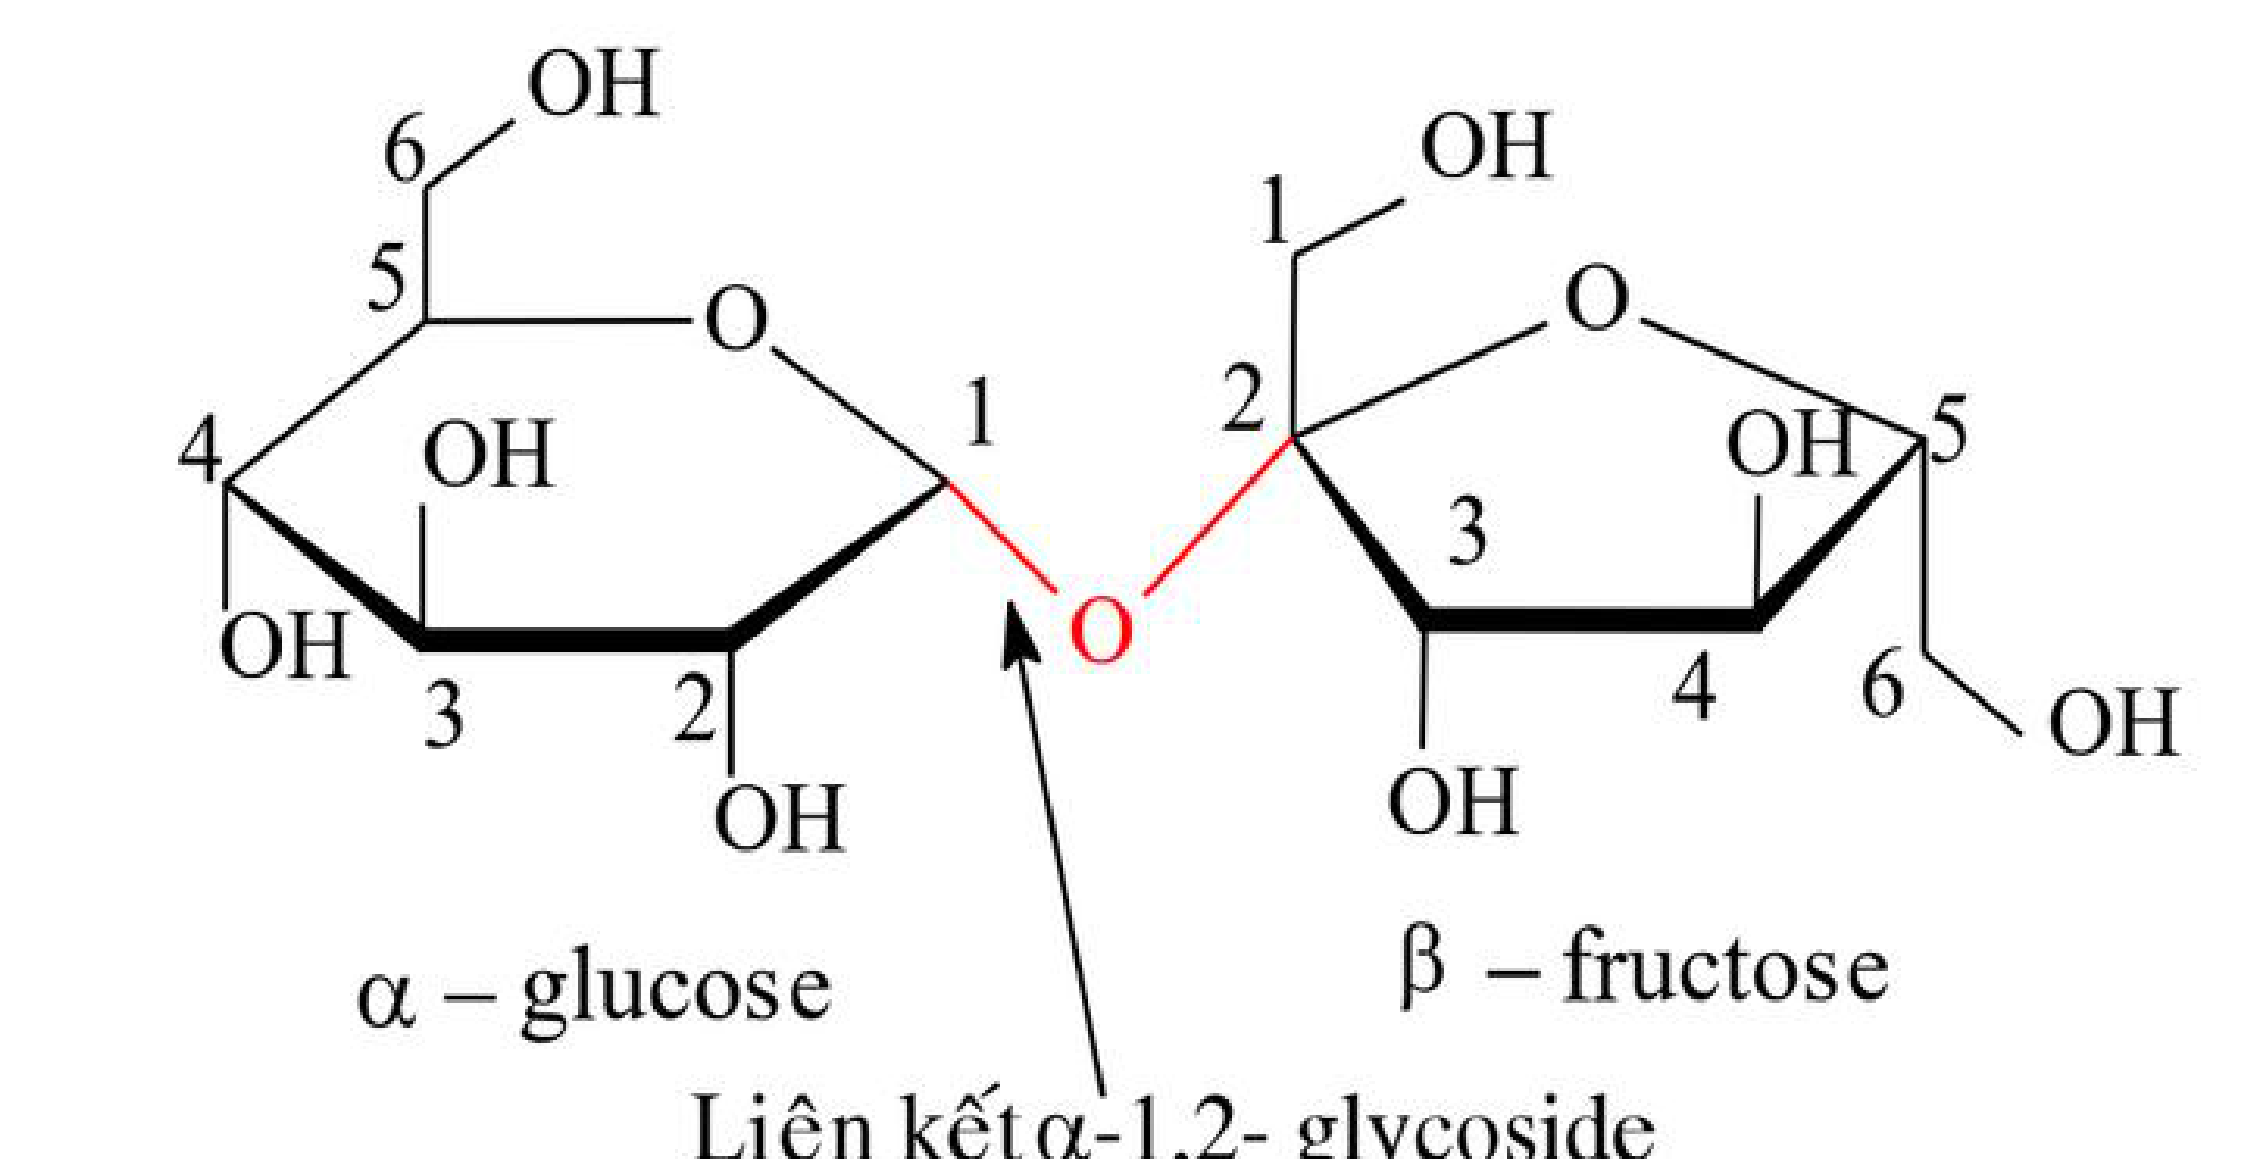
\includegraphics[width=9.5cm]{images_crop_de06/p2_cau2_saccharose.png}
\end{center}
\item \textbf{Khả năng mở vòng:}\\
- Phân tử saccharose \textbf{không thể mở vòng} được.\\
- \textit{Giải thích:} Vì nhóm \ce{-OH} hemiacetal ở carbon C1 của gốc $\alpha$-glucose và nhóm \ce{-OH} hemiketal ở carbon C2 của gốc $\beta$-fructose đều đã tham gia tạo liên kết $\alpha$-1,2-glycoside. Do đó trong phân tử saccharose không còn nhóm \ce{-OH} hemiacetal hay hemiketal tự do nào để mở vòng tạo lại nhóm chức carbonyl (\ce{-CHO} hoặc \ce{>C=O}). Phân tử chỉ tồn tại cố định ở dạng mạch vòng khép kín.
\end{enumerate}}
\end{ex}

\begin{ex}
Thủy phân hết $m$ gam tetrapeptide Ala-Ala-Ala-Ala thu được hỗn hợp gồm 44,5 gam Ala, 24 gam Ala-Ala và 46,2 gam Ala-Ala-Ala. Xác định giá trị $m$.
\loigiai{
\begin{enumerate}[label=\textbf{\arabic*.}]
\item \textbf{Khối lượng mol các chất:}\\
- $\text{Ala}~(\ce{C3H7O2N}): M = 89\,\text{g/mol}$.\\
- $\text{Ala-Ala}~(\text{Ala}_2): M = 89 \times 2 - 18 = 160\,\text{g/mol}$.\\
- $\text{Ala-Ala-Ala}~(\text{Ala}_3): M = 89 \times 3 - 36 = 231\,\text{g/mol}$.\\
- Tetrapeptide $\text{Ala}_4: M = 89 \times 4 - 54 = 302\,\text{g/mol}$.
\item \textbf{Số mol các sản phẩm thu được:}\\
- $n_{\text{Ala}} = \dfrac{44{,}5}{89} = 0{,}5\,\text{mol}$.\\
- $n_{\text{Ala-Ala}} = \dfrac{24}{160} = 0{,}15\,\text{mol}$.\\
- $n_{\text{Ala-Ala-Ala}} = \dfrac{46{,}2}{231} = 0{,}2\,\text{mol}$.
\item \textbf{Bảo toàn mắt xích Ala:}\\
Tổng số mol mắt xích Ala trong các sản phẩm thu được:\\
$n_{\text{Ala (mắt xích)}} = 1 \times n_{\text{Ala}} + 2 \times n_{\text{Ala-Ala}} + 3 \times n_{\text{Ala-Ala-Ala}}$\\
$n_{\text{Ala (mắt xích)}} = 1 \times 0{,}5 + 2 \times 0{,}15 + 3 \times 0{,}2 = 0{,}5 + 0{,}3 + 0{,}6 = 1{,}4\,\text{mol}$.
\item \textbf{Số mol tetrapeptide $\text{Ala}_4$ ban đầu:}\\
Vì mỗi phân tử $\text{Ala}_4$ có 4 mắt xích Ala:\\
$n_{\text{Ala}_4} = \dfrac{n_{\text{Ala (mắt xích)}}}{4} = \dfrac{1{,}4}{4} = 0{,}35\,\text{mol}$.
\item \textbf{Khối lượng tetrapeptide $m$:}\\
$m = n_{\text{Ala}_4} \times M_{\text{Ala}_4} = 0{,}35 \times 302 = \mathbf{105{,}7\,\text{gam}}$.\\
\textbf{Đáp số:} \textbf{105,7 gam}
\end{enumerate}}
\end{ex}

\begin{center}
\textbf{---------- HẾT ----------}
\end{center}

\end{document}
